\begin{figure*}[t]
    \centering
    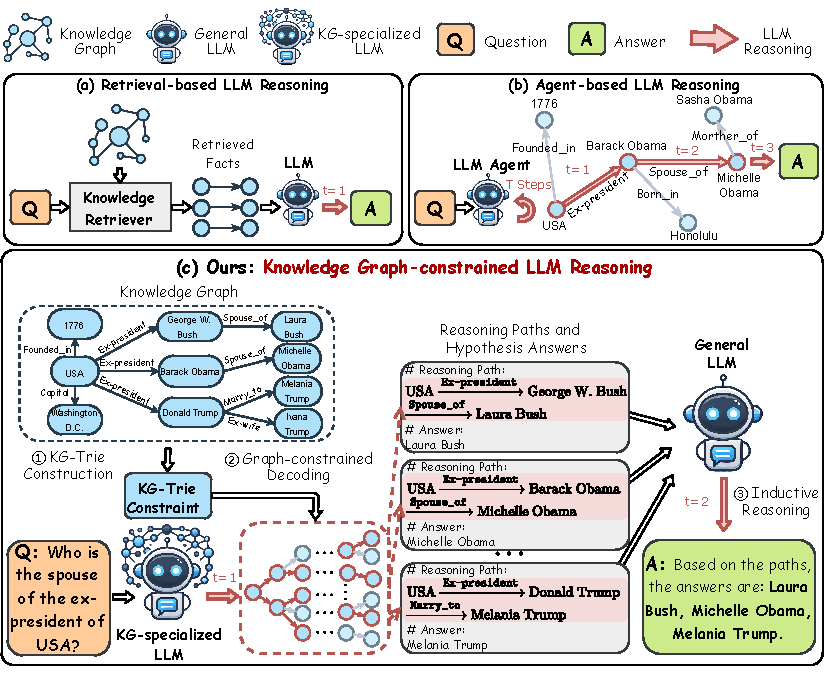
\includegraphics[width=.84\textwidth]{images/framework.pdf}
    \vspace{-.6cm}
    \caption{Illustration of existing KG-enhanced LLM reasoning paradigms and proposed graph-constrained reasoning (\ourmethod), which consists of three main components: 1) Knowledge Graph Trie Construction: building a structural index of KG to guide LLM reasoning, 2) Graph-constrained Decoding: generating KG-grounded paths and hypothesis answers using LLMs, and 3) Graph Inductive Reasoning: reasoning over multiple paths and hypotheses to derive final answers.}
    \label{fig:framework}
    \vspace{-0.5cm}
\end{figure*}



% 1) First, given a KG, we convert it into the KG-Trie, serving as a structured index to facilitate efficient reasoning path searches using LLMs. 2) Then, we design a graph-constrained decoding process that employs a lightweight KG-specialized LLM to generate multiple KG-grounded reasoning paths and hypothesis answers. This ensures the faithfulness of the reasoning process while leveraging the strong capabilities of LLMs to efficiently explore reasoning paths within KGs. 3) Finally, we input the generated reasoning paths and hypothesis answers into a powerful general LLM to utilize its inductive reasoning ability to produce final answers.
% \vspace{-.2cm}
\section{Preliminary}\label{sec:preliminary}
% \vspace{-.3cm}
% \noindent\textbf{Chain-of-Thought Reasoning (CoT)} \citep{wei2022chain} enhances the reasoning ability of LLMs by prompting LLMs to autoregressively generate a series of reasoning steps leading to the answer: $P(a|q)=P_\theta(a,z_{1,\ldots,n}|q)=P_\theta(a|q, z_{1,\ldots,n})\prod_{i=1}^{n}P_\theta(z_i|q, z_{1,\ldots,i-1})$, where $q$ denotes the input question, $a$ denotes the final answer, $z_i$ denotes the $i$-th step of the reasoning process, and $\theta$ denotes the parameters of LLMs.

\noindent\textbf{Knowledge Graphs (KGs)} represent a wealth of factual knowledge as a collection of triples: $\gG=\{(e,r,e')\in \gE\times\gR\times\gE\}$, where $\gE$ and $\gR$ denote the set of entities and relations, respectively.

\noindent\textbf{Reasoning Paths} are sequences of consecutive triples in KGs: $\vw_\vz=e_0\xrightarrow{r_1}e_1\xrightarrow{r_2}\ldots\xrightarrow{r_l}e_{l}$, where $\forall (e_{i-1}, r_i, e_i)\in \gG$.
%
The paths reveal the connections between knowledge that potentially facilitate reasoning. For example, the reasoning path: $\vw_\vz=\text{Alice}\xrightarrow{\texttt{marry\_to}}\text{Bob}\xrightarrow{\texttt{father\_of}}\text{Charlie}$ indicates that ``Alice'' is married to ``Bob'' and ``Bob'' is the father of ``Charlie''. Therefore, ``Alice'' could be reasoned to be the mother of ``Charlie''.

\noindent\textbf{Knowledge Graph Question Answering (KGQA)} is a representative reasoning task with the assistance of KGs. Given a natural language question $q$ and a KG $\gG$, the task aims to design a function $f$ to reason answers $a\in\gA$ based on knowledge from $\gG$, i.e., $a=f(q,\gG)$. 
The entities $e_q\in\gE_q$ mentioned in $q$ are linked to the corresponding entities in $\gG$, i.e., $\gE_q\subseteq\gE$.
% Following previous works \citep{sun2019pullnet,jiang2022unikgqa}, we assume the entities $e_q\in\gT_q$ mentioned in $q$ and answers $a\in\gA_q$ are labeled and linked to the corresponding entities in $\gG$, i.e., $\gT_q,\gA_q\subseteq\gE$.

\RE{
\noindent\textbf{KG-constrained Zero-hallucination.} As facts in KGs are usually verified, making them a reliable source for assessing the faithfulness of LLM reasoning \citep{nguyen-etal-2024-direct}. In this paper, we define KG-constrained zero hallucinations as the LLM generated reasoning paths can be fully grounded within KGs, ensuring the alignment of reasoning process with real-world facts.
}